\chapter{预备知识}\label{chapt:preliminary}
本章介绍的是本文中用到的一些相关的预备知识。
\section{模型检测}
\subsection{模型检测的一般流程}
如图\ref{modelchecking:overview}所示,利用模型检测方法来对计算机软硬件系统进行形式化验证的一般流程可总结为:
\begin{enumerate}
	\item 针对要验证的软硬件系统建立一个形式化模型;
	\item 将要验证的性质用一种逻辑公式表示出来;
	\item 利用算法来判断要验证的性质是否在给定的形式化模型上是可满足的,如果要验证的性质在给定的形式化模型上可满足,则输出$True$,否则输出$False$并给出反例来说明性质不满足的原因。
%	\item 当验证结束后,输出验证结果,
\end{enumerate}
%在完成这两步之后,则需要利用计算机算法来判断所描述的性质在给出的形式化模型上是否可满足。
\begin{figure}[h!]
	\centering
	\caption{模型检测流程}
	\label{modelchecking:overview}
	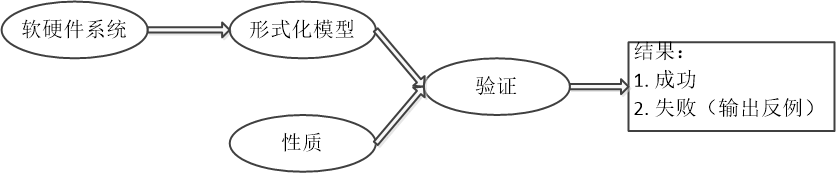
\includegraphics[width=12cm]{Img/model_checking_overview.png}
	
\end{figure}
\subsection{形式化模型}
在模型检测中,要验证软硬件系统的性质,首先必须针对该系统建立一个形式化模型。在这里,一个形式化模型通常指的是一个Kripke模型。模型检测中的经典的Kripke模型的定义如下:
%在现实世界中,系统的形式化模型既可以用常用的编程语言(比如C以及Java等),也可以利用模型检测工具的输入语言来描述。虽然

%,而模型的性质通常用时序逻辑公式来表示。模型检测的基本流程则可概述为:对于一个给定的Kripke模型$M$和一个时序逻辑公式$f$,判断Kripke模型是否满足性质$f$,如果是则返回$true$,否则返回一个反例来代表性质不满足的原因。

\begin{definition}[经典的Kripke模型]
	设$AP$是一个有穷的原子命题集合,$AP$上的一个经典的Kripke模型可表示为一个四元组$M=(S,S_0,\lra,L)$,其中
	\begin{enumerate}
		\item $S$是一个有穷状态集合;
		\item $S_0\subseteq S$是初始状态集合;
		\item $\lra\subseteq S\times S$是一个二元关系,同时对$\forall s\in S$,都存在一个状态$s'\in S$使得$s\lra s'$;
		\item $L:S\rightarrow 2^{AP}$是一个标签函数,$L$将$S$中的每个状态都映射到一个$AP$的子集。
	\end{enumerate}
\end{definition}
在Kripke模型$M$中,我们将一条从状态$s$出发的一条无穷序列$\pi=s_0,s_1,...$称为一条\textit{路径},其中$s=s_0$,而且对于任意$i\ge 0$,都有$s_i\lra s_{i+1}$。

\subsection{性质}
Kripke模型的性质通常用时序逻辑公式来表示,而根据所需要描述的系统性质类型的不同,常用的时序逻辑有线性时序逻辑\textsf{LTL}\cite{Pnueli77}、计算树逻辑\CTL{}\cite{ClarkeE08}以及\textsf{LTL}与\textsf{CTL}的超集\textsf{CTL$^*$}\cite{EmersonH86}。
本文着重介绍计算树逻辑\CTL{}以及基于\CTL{}的扩展。
%\subsubsection{\textsf{LTL}}

%\subsubsection{\CTL{}}
\begin{definition}[计算树逻辑\CTL{}]
	设$AP$是一个有穷的原子命题集合,那么基于$AP$的所有\CTL{}公式可表示为:
	$$\phi ::= \top\mid\bot\mid P\mid \neg\phi\mid \phi_1\wedge\phi_2\mid\phi_1\vee\phi_2\mid AX\phi\mid EX\phi\mid AF\phi\mid EG\phi\mid A[\phi_1 R \phi_2]\mid E[\phi_1 U \phi_2]$$
	其中$\top$表示永真,$\bot$表示永假,$P\in AP$是一个原子命题。
\end{definition}
然后,我们可以在经典的Kripke模型上定义\CTL{}的语义。
\begin{definition}[\CTL{}的语义]
	设$M=(S,S_0,\lra,L)$是在$AP$上的一个经典的Kripke模型。我们用$M,s\models \phi$来表示\CTL{}公式$\phi$在状态$s$上满足。$\models$的归纳定义如下。
	\begin{itemize}
		\item $M,s\models \top$永远成立;
		\item $M,s\models \bot$永远不成立;
		\item $M,s\models P$当且仅当$p\in L(s)$;
		\item $M,s\models \neg\phi$当且仅当$M,s\not\models\phi$;
		\item $M,s\models \phi_1\wedge\phi_2$当且仅当$M,s\models\phi_1$且$M,s\models\phi_2$;
		\item $M,s\models \phi_1\vee\phi_2$当且仅当$M,s\models\phi_1$或$M,s\models\phi_2$;
		\item $M,s\models AX\phi$当且仅当$\forall s'\in \{s'\in S\mid s\lra s'\}$,$M,s'\models \phi$;
		\item $M,s\models EX\phi$当且仅当$\exists s'\in \{s'\in S\mid s\lra s'\}$,$M,s'\models \phi$;
		\item $M,s\models AF\phi$当且仅当对于任意从$s$出发的路径$s_0,s_1,...$都存在$i\ge 0$使得$M,s_i\models \phi$;
		\item $M,s\models AF\phi$当且仅当存在从$s$出发的路径$s_0,s_1,...$使得对于任意$i\ge 0$都有$M,s_i\models \phi$;
		\item $M,s\models A[\phi_1 R\phi_2]$当且仅当对于任意从$s$出发的路径$s_0,s_1,...$:如果存在$j\ge 0$使得$M,s_j\models\phi_1$成立,那么对于所有的$0\le i\le j$都有$M,s_i\models\phi_2$成立;否则,对任意$i\ge 0$都有$M,s_i\models\phi_2$成立。
		\item $M,s\models E[\phi_1 U\phi_2]$当且仅当存在从$s$出发的路径$s_0,s_1,...$使得:存在$j\ge 0$使得$M,s_j\models\phi_2$成立且对于所有的$0\le i< j$都有$M,s_i\models\phi_1$成立;
	\end{itemize}
\end{definition}

\subsection{验证}
对于给定的Kripke模型$M$,状态$s$和\CTL{}公式$\phi$,\CTL{}模型检测的验证过程即判断$M,s\models \phi$是否成立。如果要验证的性质在给定的形式化模型上可满足,则输出$True$,否则输出$False$并给出反例来说明性质不满足的原因。对于以“$A*$”形式模态词开头的\CTL{}公式,一个反例指的是一条路径。比如如果$M,s\not\models AF\phi$,那么模型检测工具给出的反例是一条无穷路径,其中对于该无穷路径上的任意状态$s'$都有$M,s'\not\models \phi$。对于以“$E*$”形式模态词开头的\CTL{}公式,一个反例指的是一系列路径。比如如果$M,s\not\models E[\phi_1 U\phi_2]$,那么模型检测工具给出的反例是所有满足以下条件的路径:即以$s$为起始状态,而且如果该路径为有穷路径,那么对于该路径上的最后一个状态$s'$有$M,s'\not\models\phi_1$且$M,s'\not\models\phi_2$,同时对于该路径上的任意其他状态(如果存在)$s''$有$M,s''\models \phi_1$;如果该路径为无穷路径,那么对于该路径上的任意状态$s'$有$M,s'\models \phi_1$且$M,s'\not\models \phi_2$。另外,值得注意的是,当要验证的\CTL{}公式以“$E*$”形式模态词开头时,一个更自然的选择是:当该公式在给定的Kripke模型上不满足时不给出反例,而当该公式在给定的Kripke模型上满足时,给出一个证据(witness)来说明该公式可满足的原因\cite{BaierKatoen08}。比如,如果$M,s\models E[\phi_1 U\phi_2]$,那么模型检测工具通常给出一个以$s$为起始状态的有穷路径,使得对于该路径上的最后一个状态$s'$有$M,s'\models\phi_2$,而且对于该路径上的任意其他状态(如果存在)$s''$有$M,s''\models\phi_1$。满足这个条件的路径即为$M,s\models E[\phi_1 U\phi_2]$的证据。


\section{相继式演算(Sequent Calculus)}
在本文中,我们需要用到相继式演算的概念。在数理逻辑与证明论中,相继式演算指的是一系列具有特定形式的证明系统:每个证明判断(proof judgement)包含两部分:上下文(context)和命题(proposition)。在相继式演算中,证明判断被称为相继式(sequent)。例如,在$\Gamma\vdash A$形式的相继式中,命题集合$\Gamma$是上下文,$A$是命题。$\Gamma\vdash A$可非形式化地解释为:若$\Gamma$中所有的命题均为真,那么命题$A$为真。
在某些相继式演算中,$\vdash$后也可有多个命题,被称为多结论的相继式演算,比如$\Gamma\vdash A_1,...,A_n$,这种形式的相继式可非形式化地解释为:若$\Gamma$中所有命题均为真,那么$A_1,...,A_n$中存在某个为真的命题。在本文中,我们用到的是单结论的相继式演算,即每个相继式中$\vdash$之后只有一个命题。

下面,我们在一阶逻辑中形式化地解释相继式演算的概念。在这之前,我们先介绍一阶语言、项、命题以及相继式的概念。
\begin{definition}[一阶语言]
	一个一阶语言$\mathcal{L}$可用一个三元组$(\mathcal{S}, \mathcal{F}, \mathcal{P})$来表示,其中
	\begin{itemize}
		\item $\mathcal{S}$是一个非空的有穷集合,集合的元素被称为项的类别(term sort);
		\item $\mathcal{F}$是函数符号的集合;
		\item $\mathcal{P}$是谓词符号的集合。
	\end{itemize}
	每个函数符号都有一个元数(arity),用$S$上的一个$(n+1)$-元组来表示;每个谓词符号也具有一个元数,用$S$上的一个$n$-元组来表示。
	
\end{definition}

\begin{definition}[项]
	假设一个一阶语言$\mathcal{L}=(\mathcal{S}, \mathcal{F}, \mathcal{P})$,并且令$(\mathcal{V}_s)_{s\in S}$为一系列无穷的变量集合,并由项的类别$s$区分开来。$\mathcal{L}$中项的集合由如下的方式归纳定义:
		\begin{itemize}
		\item 对于每个类别$s\in S$,$\mathcal{V}_s$中的每个变量都是具有类别$s$的项;
		\item 对于每个函数符号$f\in\mathcal{F}$,假设$f$的元数为$(s_1,...,s_n, s')$,那么对于任意$n$个项$t_1,...,t_n$,其中$t_i$的类别为$s_i$,$f(t_1,...,t_n)$是具有类别$s'$的项。
	\end{itemize}
\end{definition}

\begin{definition}[命题]
		假设一个一阶语言$\mathcal{L}=(\mathcal{S}, \mathcal{F}, \mathcal{P})$,并且令$(\mathcal{V}_s)_{s\in S}$为一系列无穷的变量集合,并由项的类别$s$区分开来。那么$\mathcal{L}$中基于$(\mathcal{V}_s)_{s\in S}$的命题的集合由如下的方式归纳定义:
		\begin{itemize}
			\item 对于每个谓词符号$P\in\mathcal{P}$,假设$P$的元数为$(s_1,...,s_n)$,那么对于任意$n$个项$t_1,...,t_n$,其中$t_i$的类别为$s_i$,$P(t_1,...,t_n)$是一个命题;
			\item $\top$和$\bot$均为命题;
			\item 如果$A$是一个命题,那么$\neg A$也是一个命题;
			\item 如果$A$和$B$均为命题,那么$A\wedge B$、$A\vee B$、$A\Rightarrow B$都是命题;
			\item 如果$A$是一个命题,且$x$是一个变量,那么$\forall x A$和$\exists x A$均为命题。
		\end{itemize}
	
\end{definition}
在命题中,量词符号$\forall$、$\exists$被用来绑定变量:对于$\forall x A$和$\exists y B$形式的命题,量词$\forall$绑定$A$中自由出现的变量$x$,量词$\exists$绑定$B$中自由出现的变量$y$,而一个变量在命题中自由出现指的是该变量在该命题中不被任何量词绑定。一个命题是闭命题(closed proposition)指的是该命题中不存在自由出现的变量。

%\begin{remark}
	对于一个一阶语言$\mathcal{L}=(\mathcal{S}, \mathcal{F}, \mathcal{P})$,如果$\mathcal{S}$只包含一个元素,那么$\mathcal{L}$中函数符号和谓词符号的元数可简单地表示为自然数,即参数的个数。
%\end{remark}

接下来,我们介绍一种方法来区分可证的命题(比如$\exists x(x=0+1)$)以及不可证的命题(比如$\exists x(0=x+1)$)。在这里,我们将可证的命题的集合利用规则进行归纳定义。命题的可证性是基于相继式的概念,相继式的证明规则如图\ref{preliminary:sequent:calculus}所示。

%命题的证明是基于相继式演算的。
\begin{definition}[相继式]
	一个相继式被表示为一个具有$\Gamma\vdash A$形式的二元组,其中$\Gamma$是一个命题的有穷集合,$A$是一个命题。
\end{definition}

\begin{definition}[相继式的证明]
	相继式$\Gamma\vdash A$的一个证明是一棵树:根节点被标记为$\Gamma\vdash A$,而且对于这棵树上所有标记为$\Gamma'\vdash B$的节点,如果该节点的所有子节点分别被标记为$\Gamma_1\vdash C_1,...,\Gamma_n\vdash C_n$,那么由相继式的证明规则可以从$\Gamma_1\vdash C_1,...,\Gamma_n\vdash C_n$推导出$\Gamma'\vdash B$;如果标记为$\Gamma'\vdash B$的节点为叶节点,那么$B\in \Gamma'$,或者$B=\top$,或者$B$具有$B_1\vee\neg B_1$形式。
\end{definition}

\begin{definition}[理论]
	一个理论指的是一个闭命题的有穷或无穷集合,理论中的每个元素被称为公理。
\end{definition}
%下面,我们来说明如何定义一个可证的命题。
\begin{definition}[可证的命题]
	一个命题在理论$\mathcal{T}$中是可证的指的是存在$\mathcal{T}$的有穷子集$\Gamma$使得相继式$\Gamma\vdash A$存在一个证明。
	
	一个可证的命题也可被称为一个定理。
\end{definition}
\begin{figure}[!h]
	\centering
		\small
		\caption{相继式演算的规则}
		\label{preliminary:sequent:calculus}
		\renewcommand\arraystretch{1.7}
			\begin{tabular}{|ll|}
			\hline
			$$
			\infer[A\in\Gamma]{\Gamma\vdash A}{}
			$$
			&
			$$
			\infer[\top\mathsf{-intro}]{\Gamma\vdash\top}{}
			$$\\
			$$
			\infer[\bot\mathsf{-elim}]{\Gamma\vdash A}{\Gamma\vdash \bot}
			$$
			&
			$$
			\infer[\wedge\mathsf{-intro}]{\Gamma\vdash A\wedge B}{\Gamma\vdash A & \Gamma\vdash B}
			$$\\
			$$
			\infer[\wedge\mathsf{-elim}]{\Gamma\vdash A}{\Gamma\vdash A\wedge B}
			$$
			&
			$$
			\infer[\vee\mathsf{-intro}]{\Gamma\vdash A\vee B}{\Gamma\vdash A}
			$$\\
			$$
			\infer[\vee\mathsf{-intro}]{\Gamma\vdash A\vee B}{\Gamma\vdash B}
			$$
			&
			$$
			\infer[\vee\mathsf{-elim}]{\Gamma\vdash C}{\Gamma\vdash A\vee B & \Gamma,A\vdash C & \Gamma, B\vdash C}
			$$\\
			$$
			\infer[\Rightarrow\mathsf{-intro}]{\Gamma\vdash A\Rightarrow B}{\Gamma, A\vdash B}
			$$
			&
			$$
			\infer[\Rightarrow\mathsf{-elim}]{\Gamma\vdash B}{\Gamma\vdash A\Rightarrow B & \Gamma\vdash A}
			$$\\
			$$
			\infer[\neg\mathsf{-intro}]{\Gamma\vdash\neg A}{\Gamma,A\vdash \bot}
			$$
			&
			$$
			\infer[\neg\mathsf{-elim}]{\Gamma\vdash \bot}{\Gamma\vdash A & \Gamma\vdash \neg A}
			$$\\
			$$
			\infer[{\forall\mathsf{-intro},}\;{x\;\mathsf{not}\;\mathsf{free}\;\mathsf{in}\;\Gamma}]{\Gamma\vdash\forall x A}{\Gamma\vdash A}
			$$
			&
			$$
			\infer[\forall\mathsf{-elim}]{\Gamma\vdash (t/x)A}{\Gamma\vdash A}
			$$\\
			$$
			\infer[\exists\mathsf{-intro}]{\Gamma\vdash\exists x A}{\Gamma\vdash (t/x)A}
			$$
			&
			$$
			\infer[\exists\mathsf{-elim,}x\;\mathsf{not}\;\mathsf{free}\;\mathsf{in}\;\Gamma,B]{\Gamma\vdash B}{\Gamma\vdash\exists x A & \Gamma,A\vdash B}
			$$\\
			$$
			\infer[\mathsf{excluded}\;\mathsf{middle}]{\Gamma\vdash A\vee\neg A}{}
			$$&{}
			\\
			\hline
		\end{tabular}
	
\end{figure}

\section{信息可视化}
信息可视化是一个研究如何利用计算机图形学技术将数据中的抽象信息可视化的研究领域。抽象信息的可视化表达可以用来帮助人们揭示数据的隐匿模式,用来帮助更好地理解和发现数据中的规律。得益于计算机图形学理论的日益成熟以及计算机硬件的飞速发展,信息可视化系统能可视化越来越大的数据集以及越来越复杂的数据结构,并在许多行业中发挥着举足轻重的作用。比如,在知识管理领域,信息可视化系统可以用来研究不同学科领域知识之间的关系和演化\cite{ZHHW16};在城市交通系统的研究中,信息可视化系统可以将城市的公共交通工具的卫星定位数据进行可视化,以帮助人们研究和改善公共交通的效率\cite{FYL15}。绝大多数信息可视化系统是基于\textsf{OpenGL}的。
\textsf{OpenGL},全称Open Graphics Library,是一个跨编程语言并且跨平台的编程接口的标准。在计算机系统中,通常由显卡提供\textsf{OpenGL}的实现。一个典型的基于\textsf{OpenGL}的3D图形的显示过程为:首先,用户程序通过调用\textsf{OpenGL}的绘图\textsf{API}(Application Programming Interface)来定义一组要显示的图形的数据和命令,并将这些数据和命令存储在计算机的主内存(RAM)中;然后,计算机的中央处理器(CPU)会通过CPU时钟将这些数据和命令发送到显卡的显存(VRAM)中,并在图形处理器(GPU)的控制下完成图形的渲染;最后,图形渲染的结果会被存入帧缓冲区中,而帧缓冲区中的帧则最终被发送到计算机的显示器上,并显示出结果。

